%% This file was auto-generated by IPython, do NOT edit
%% Conversion from the original notebook file:
%% 01_Introducing_Python.ipynb
%%
\documentclass[11pt,english]{article}

%% This is the automatic preamble used by IPython.  Note that it does *not*
%% include a documentclass declaration, that is added at runtime to the overall
%% document.

\usepackage{amsmath}
\usepackage{amssymb}
\usepackage{graphicx}
\usepackage{ucs}
\usepackage[utf8x]{inputenc}

% needed for markdown enumerations to work
\usepackage{enumerate}

% Slightly bigger margins than the latex defaults
\usepackage{geometry}
\geometry{verbose,tmargin=3cm,bmargin=3cm,lmargin=2.5cm,rmargin=2.5cm}

% Define a few colors for use in code, links and cell shading
\usepackage{color}
\definecolor{orange}{cmyk}{0,0.4,0.8,0.2}
\definecolor{darkorange}{rgb}{.71,0.21,0.01}
\definecolor{darkgreen}{rgb}{.12,.54,.11}
\definecolor{myteal}{rgb}{.26, .44, .56}
\definecolor{gray}{gray}{0.45}
\definecolor{lightgray}{gray}{.95}
\definecolor{mediumgray}{gray}{.8}
\definecolor{inputbackground}{rgb}{.95, .95, .85}
\definecolor{outputbackground}{rgb}{.95, .95, .95}
\definecolor{traceback}{rgb}{1, .95, .95}

% Framed environments for code cells (inputs, outputs, errors, ...).  The
% various uses of \unskip (or not) at the end were fine-tuned by hand, so don't
% randomly change them unless you're sure of the effect it will have.
\usepackage{framed}

% remove extraneous vertical space in boxes
\setlength\fboxsep{0pt}

% codecell is the whole input+output set of blocks that a Code cell can
% generate.

% TODO: unfortunately, it seems that using a framed codecell environment breaks
% the ability of the frames inside of it to be broken across pages.  This
% causes at least the problem of having lots of empty space at the bottom of
% pages as new frames are moved to the next page, and if a single frame is too
% long to fit on a page, will completely stop latex from compiling the
% document.  So unless we figure out a solution to this, we'll have to instead
% leave the codecell env. as empty.  I'm keeping the original codecell
% definition here (a thin vertical bar) for reference, in case we find a
% solution to the page break issue.

%% \newenvironment{codecell}{%
%%     \def\FrameCommand{\color{mediumgray} \vrule width 1pt \hspace{5pt}}%
%%    \MakeFramed{\vspace{-0.5em}}}
%%  {\unskip\endMakeFramed}

% For now, make this a no-op...
\newenvironment{codecell}{}

 \newenvironment{codeinput}{%
   \def\FrameCommand{\colorbox{inputbackground}}%
   \MakeFramed{\advance\hsize-\width \FrameRestore}}
 {\unskip\endMakeFramed}

\newenvironment{codeoutput}{%
   \def\FrameCommand{\colorbox{outputbackground}}%
   \vspace{-1.4em}
   \MakeFramed{\advance\hsize-\width \FrameRestore}}
 {\unskip\medskip\endMakeFramed}

\newenvironment{traceback}{%
   \def\FrameCommand{\colorbox{traceback}}%
   \MakeFramed{\advance\hsize-\width \FrameRestore}}
 {\endMakeFramed}

% Use and configure listings package for nicely formatted code
\usepackage{listingsutf8}
\lstset{
  language=python,
  inputencoding=utf8x,
  extendedchars=\true,
  aboveskip=\smallskipamount,
  belowskip=\smallskipamount,
  xleftmargin=2mm,
  breaklines=true,
  basicstyle=\small \ttfamily,
  showstringspaces=false,
  keywordstyle=\color{blue}\bfseries,
  commentstyle=\color{myteal},
  stringstyle=\color{darkgreen},
  identifierstyle=\color{darkorange},
  columns=fullflexible,  % tighter character kerning, like verb
}

% The hyperref package gives us a pdf with properly built
% internal navigation ('pdf bookmarks' for the table of contents,
% internal cross-reference links, web links for URLs, etc.)
\usepackage{hyperref}
\hypersetup{
  breaklinks=true,  % so long urls are correctly broken across lines
  colorlinks=true,
  urlcolor=blue,
  linkcolor=darkorange,
  citecolor=darkgreen,
  }

% hardcode size of all verbatim environments to be a bit smaller
\makeatletter 
\g@addto@macro\@verbatim\small\topsep=0.5em\partopsep=0pt
\makeatother 

% Prevent overflowing lines due to urls and other hard-to-break entities.
\sloppy

\begin{document}

\section{Python in HPC}


\subsection{Supercomputing 2012}

Presenters:


\noindent {\bf Andy R. Terrel, PhD}\\
Texas Advanced Computing Center\\
University of
Texas at Austin\\[2em]

\noindent {\bf Travis Oliphant, PhD}\\
Continuum Analytics\\[2em]

\noindent {\bf Aron Ahmadia, PhD}\\
Supercomputing Laboratory\\
King Abdullah University of Science and Technoglogy\\[2em]
\begin{center}

\href{http://creativecommons.org/licenses/by/3.0/deed.en\_US}{
\includegraphics{figures/creative_commons_logo.png}}\\[2em]

\noindent Python in HPC Tutorial by Terrel, Oliphant, and Ahmadia is licensed
under a Creative Commons Attribution 3.0 Unported License. \\[2em]

\href{http://www.tacc.utexas.edu}{
\includegraphics[scale=0.8]{figures/TACC_logo.png}} \qquad
\href{http://www.continuum.io}{
\includegraphics[scale=.3]{figures/continuum.png}} \qquad
\href{http://www.kaust.edu.sa/}{
\includegraphics[scale=.3]{figures/kaust.png}}
\end{center}

\newpage

\subsection{Updated Tutorial}

These presentation materials are being continuously updated as we refine
and improve our demonstrats. To get the latest version of this tutorial
you can:

\begin{enumerate}[1)]
\item
  Download a zip or tar ball from the
  \href{https://github.com/aterrel/HPCPythonSC2012/tags}{github SC2012
  tag}:

  wget --no-check-certificate
  https://github.com/aterrel/HPCPythonSC2012/zipball/SC2012
\item
  Checkout from git

  git clone https://github.com/aterrel/HPCPythonSC2012.git
\item
  View the html version on
  \href{http://nbviewer.ipython.org/urls/raw.github.com/aterrel/HPCPythonSC2012/master/01_Introducing_Python.ipynb}{nbviewer}.
\item
  As a last resort, head to https://github.com/aterrel/HPCPythonSC2012
  for updated instructions (see the README at the bottom of the page).
\end{enumerate}

\newpage
\subsection{Interacting with the Tutorial Slides}

This tutorial is an interactive worksheet designed to encourage you to
try out the lessons during the demonstration. If you are looking at the
pdf version, we encourage you to download the updated version (see
previous slide) and try the interactive version.

To run the interactive version, you need a good Python environment
including:

\begin{itemize}
\item
  IPython version \textgreater{}= 13.0
\item
  Numpy version \textgreater{}= 1.5
\item
  Scipy
\item
  Matplotlib
\end{itemize}

Move to the directory containing the tarball and execute:

\begin{verbatim}
$ ipython notebook --pylab=inline
\end{verbatim}

We heartily endorse the
\href{http://www.enthought.com/products/epd\_free.php}{Free Enthought
Python Distribution}.

\newpage
\subsection{Introduction to Python (This Notebook)}

\subsubsection{Objectives}

\begin{enumerate}[1.]
\item
  You will understand how scripting languages fit into the toolbox of a
  computational scientist.
\item
  You will see why Python is a powerful choice
\item
  You will get a taste of Python for actual scientific computing
\end{enumerate}

The first part of this introduction is adapted from \emph{Python
Scripting for Computational Science} by Hans Petter Langtangen and is
based on material from Nathan Collier.

\subsection{Scripting vs Traditional programming}

In traditional programming, large applications are typically written at
a low level. Scripting by contrast is programming at a very high level
with flexible languages.

\begin{quote}
Traditional programming: fortran, c, c++, c\#, java

Scripting: python, perl, ruby, (matlab)
\end{quote}

A major thrust of scripting is that you can automate many tasks that
otherwise you would do by hand.

\newpage
\subsection{Has this ever happened to you?}

\subsubsection{Scenario 1}

You are working on data for a presentation your advisor is giving at a
conference. At the last minute, you realize that there is a major bug in
your code and you need to regenerate all the images and graphs that you
have given him. You spend 30 minutes regenerating the data and 6 hours
regenerating the graphs because you had them in Excel and had done them
by hand.

\subsubsection{Scenario 2}

You are working on your thesis and as you near the finish you review
some graphs you generated months earlier and you aren't sure if they are
now completely up to date. You spend half a day locating the old code
that you wrote on your second laptop and hours more again creating and
polishing the charts.

\newpage
\subsection{Buyer Beware}

Learning to automate many of these common tasks can greatly increase
your productivity (and make your research reproducible). However, beware
that there is no end to the number of different ways to do essentially
the same thing.

\begin{figure}[htbp]
\centering
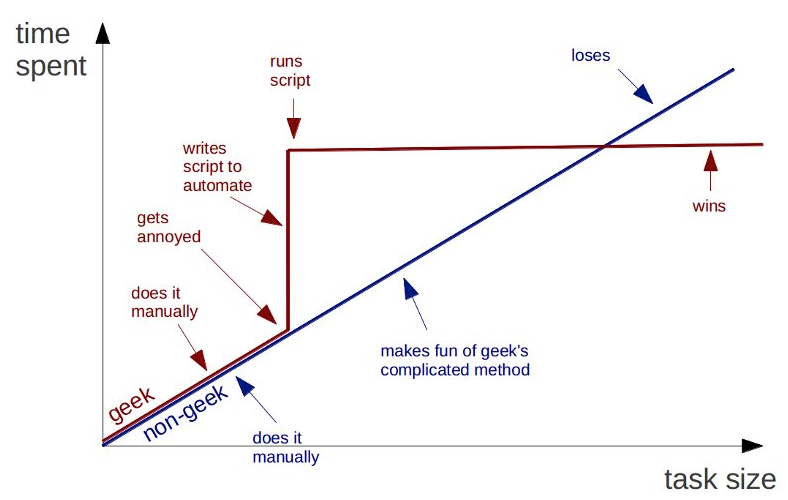
\includegraphics[scale=.5]{figures/careful.png}
\caption{Recall we want to script to SAVE time}
\end{figure}

\newpage
\subsection{Why scripting is useful}

There are perhaps many reasons, here we list a few:

\begin{itemize}
\item
  scripting languages have nicer interfaces
\item
  allow you to build your own work environment
\item
  scientific computing is more than crunching numbers
\item
  easier creation of GUIs and demos
\item
  create modern interfaces to old codes
\item
  allow you test interactively
\item
  cleaner, shorter, easy to read code
\end{itemize}

\newpage
\subsection{Is Python \textgreater{} MATLAB?}

\subsubsection{Similarities}

\begin{itemize}
\item
  no mandatory variable declaration (dynamic typing)
\item
  simple and easy to use syntax
\item
  easy creation of GUIs
\item
  merges simulation and visualization
\end{itemize}

\subsubsection{Differences}

\begin{itemize}
\item
  Python was designed to be completely open and to be integrated with
  external tools
\item
  A Python module may contain a lot of functions and classes (compared
  to many m-files)
\item
  Object-oriented programming is more convenient
\item
  Interfacing C,C++,Fortran is better supported, this is important for
  running fast, parallel code
\item
  scalar functions typically work with array arguments without changes
  to the arithmetic operators
\item
  Python is FREE and runs on any platform C does, including
  supercomputers!
\end{itemize}

\newpage
\subsection{The right tool for the job}

Many times people are looking for an easy way out. Scripting is easier
to use, but not well suited for every situation. How do you know which
tool is right for the job?

\subsubsection{Traditional programming}

\begin{itemize}
\item
  Does the application implement complex algorithms and/or data
  structures where low level control of implementation details is
  critical?
\item
  Does the application manipulate large datasets and thus the memory has
  to be carefully controlled?
\item
  Are you not likely to be changing the code once it is programmed?
\end{itemize}

\subsubsection{Scripting}

\begin{itemize}
\item
  Your application's main task is to connected existing components
\item
  The application depends on manipulating text
\item
  The design of the application is expected to change over its life
\item
  The CPU-intensive parts of your application may be migrated to C or
  Fortran
\item
  Your application is largely based on common objects found in computer
  science
\end{itemize}

\newpage
\section{Some Sample Applications}

\newpage
\subsection{Teaching the finite element method}

\subsubsection{Stiffness matrix computation}

\begin{figure}[htbp]
\centering
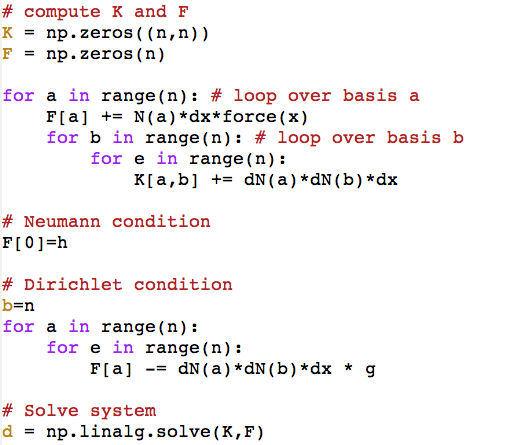
\includegraphics{figures/fem.png}
\caption{Stiffness matrix}
\end{figure}

\newpage
\subsection{Monitor program progress}

\subsubsection{Python parses a datafile and makes plots of current
progress}

\begin{figure}[htbp]
\centering
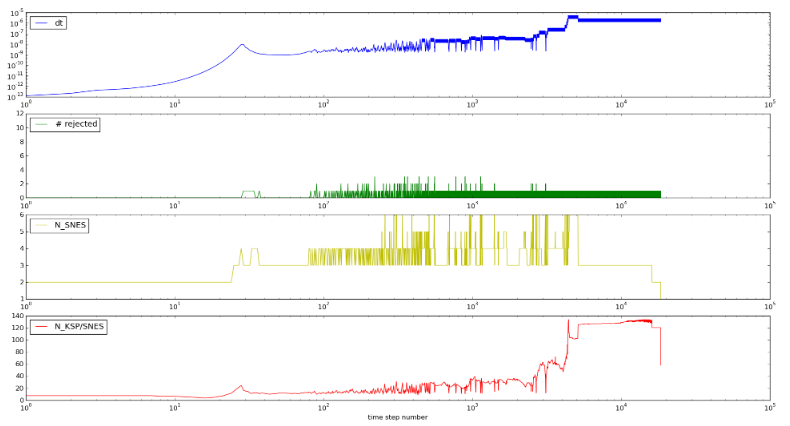
\includegraphics[scale=.5]{figures/log.png}
\caption{Log}
\end{figure}

\newpage
\subsection{Problem prototypes}

\subsubsection{Nonlinear, time dependent problem}

\begin{figure}[htbp]
\centering
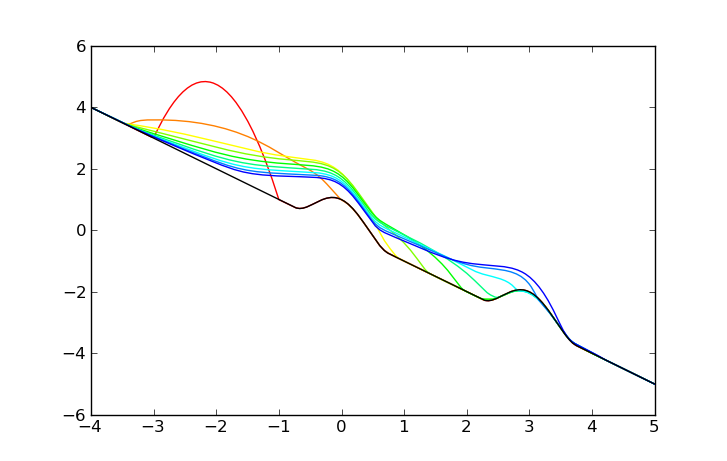
\includegraphics{figures/dsw.png}
\caption{NonLinear problem}
\end{figure}

\newpage
\subsection{Problem prototypes}

\subsubsection{Method for fitting surface to data}

\begin{figure}[htbp]
\centering
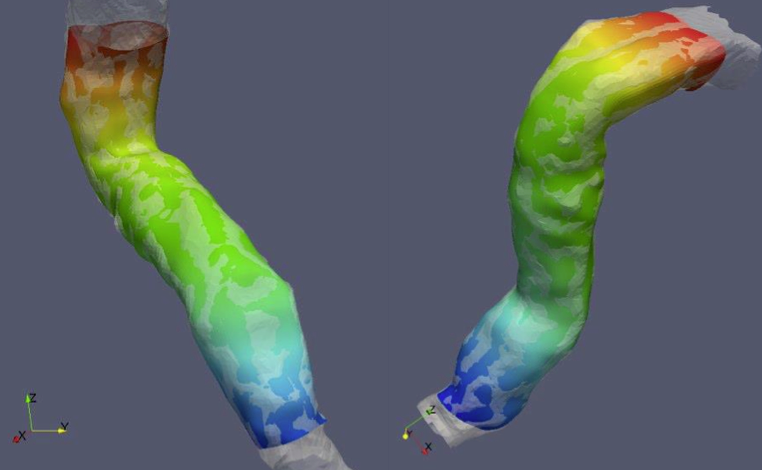
\includegraphics[scale=.5]{figures/molt.png}
\caption{Prototypes}
\end{figure}

\newpage
\subsection{Structural program}

\subsubsection{Python manages floors and columns}

\begin{figure}[htbp]
\centering
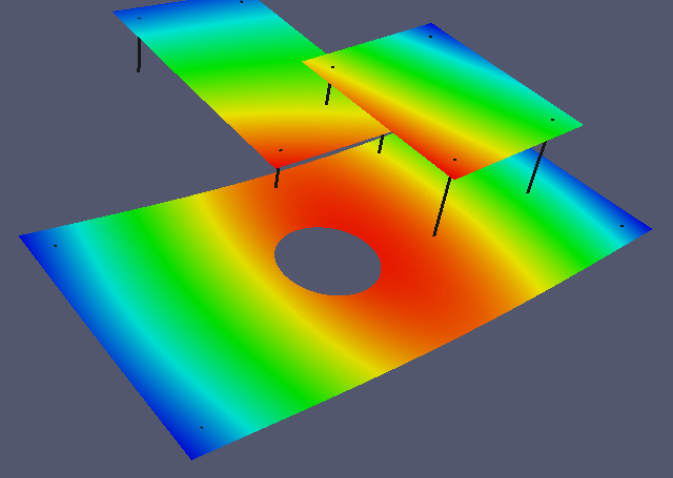
\includegraphics[scale=.5]{figures/struct.png}
\caption{Structural program}
\end{figure}

\newpage
\subsection{Auto-generation of results}

\subsubsection{Python runs C code, post-processes the results, and
generates a LaTeX table}

\begin{figure}[htbp]
\centering
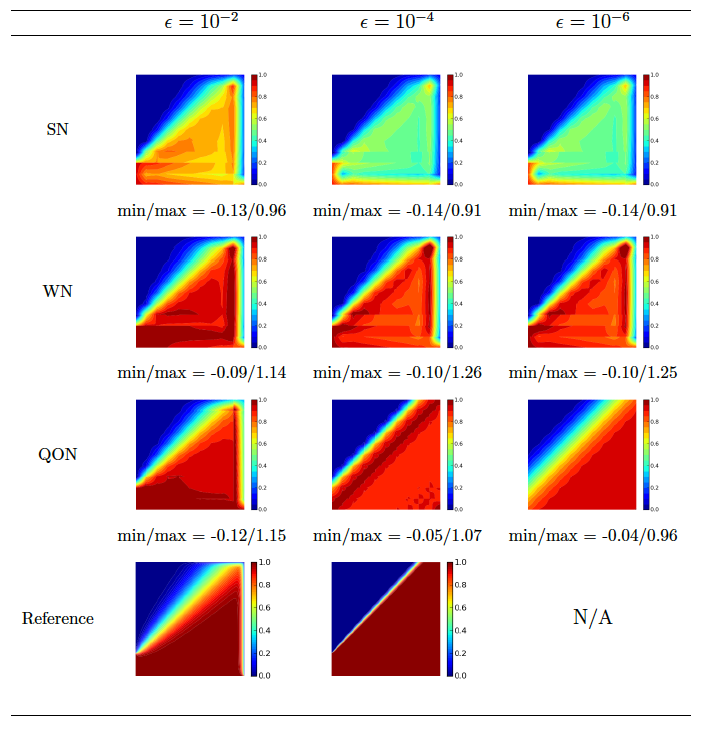
\includegraphics[scale=.5]{figures/dpg.png}
\caption{Result Generation}
\end{figure}

\newpage
\section{Beginner's Guide}

\newpage
\subsection{Script 1}

\begin{codecell}
\begin{codeinput}
\begin{lstlisting}
#!/usr/bin/env python
import math
r = math.pi / 2.0
s = math.sin(r)
print "Hello world, sin(%f)=%f" % (r,s)

\end{lstlisting}
\end{codeinput}
\begin{codeoutput}
\begin{verbatim}
Hello world, sin(1.570796)=1.000000
\end{verbatim}
\end{codeoutput}
\end{codecell}
\newpage
\subsection{Script 2}

\begin{codecell}
\begin{codeinput}
\begin{lstlisting}
import math
infile = "data/numbers"
outfile = "data/f_numbers"

f = open(infile,'r')
g = open(outfile,'w')

def func(y):
    if y >= 0.0:
        return y**5.0*math.exp(-y)
    else:
        return 0.0
    
for line in f:
    line = line.split()
    x = float(line[0])
    y = float(line[1])
    fy = func(y)
    g.write("%g %12.5e\n" % (x,fy))
    
f.close() 
g.close()

\end{lstlisting}
\end{codeinput}
\end{codecell}
\newpage
\subsection{How to format the print statement, just like C!}

\begin{figure}[htbp]
\centering
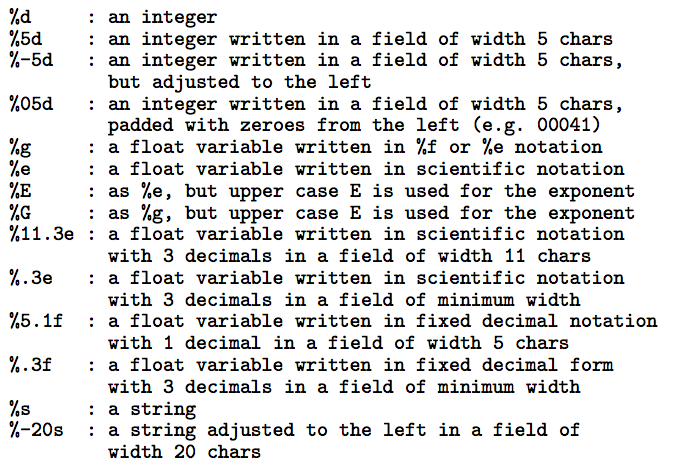
\includegraphics[scale=.75]{figures/tbl.png}
\caption{format}
\end{figure}

\newpage
\subsection{Script 3}

\begin{codecell}
\begin{codeinput}
\begin{lstlisting}
import sys,os
cmd = 'date'
output = os.popen(cmd)
lines = output.readlines()
fail = output.close()
if fail: print 'You do not have the date command'; sys.exit()
for line in lines:
    line = line.split()
    print "The current time is %s on %s %s, %s" % (line[3],line[2],line[1],line[-1])

\end{lstlisting}
\end{codeinput}
\begin{codeoutput}
\begin{verbatim}
The current time is 16:32:23 on 9 Sep, 2012
\end{verbatim}
\end{codeoutput}
\end{codecell}
\newpage
\subsection{A bib-file (see data/test.bib)}

\begin{verbatim}
@Book{Langtangen2011,
  author =    {Hans Petter Langtangen},
  title =     {A Primer on Scientific Programming with Python},
  publisher = {Springer},
  year =      {2011}
}
@Book{Langtangen2010,
  author =    {Hans Petter Langtangen},
  title =     {Python Scripting for Computational Science},
  publisher = {Springer},
  year =      {2010}
}
\end{verbatim}

\newpage
\subsection{Script 4}

\begin{codecell}
\begin{codeinput}
\begin{lstlisting}
import re
pattern1 = "@Book{(.*),"
pattern2 = "\s+title\s+=\s+{(.*)},"
for line in file('data/test.bib'):
    match = re.search(pattern1,line)
    if match: 
        print "Found a book with the tag '%s'" % match.group(1)
    match = re.search(pattern2,line)
    if match:
        print "The title is '%s'" % match.group(1)
\end{lstlisting}
\end{codeinput}
\begin{codeoutput}
\begin{verbatim}
Found a book with the tag 'Langtangen2011'
The title is 'A Primer on Scientific Programming with Python'
Found a book with the tag 'Langtangen2010'
The title is 'Python Scripting for Computational Science'
\end{verbatim}
\end{codeoutput}
\end{codecell}
\newpage
\subsection{Pattern Formation}

\begin{codecell}
\begin{codeinput}
\begin{lstlisting}
from IPython.display import clear_output


"""Pattern formation code

    Solves the pair of PDEs:
       u_t = D_1 \nabla^2 u + f(u,v)
       v_t = D_2 \nabla^2 v + g(u,v)
"""

#import matplotlib
#matplotlib.use('TkAgg')
import numpy as np
#import matplotlib.pyplot as plt
from scipy.sparse import spdiags,linalg,eye
from time import sleep

#Parameter values
Du=0.500; Dv=1;
delta=0.0045; tau1=0.02; tau2=0.2; alpha=0.899; beta=-0.91; gamma=-alpha;
#delta=0.0045; tau1=0.02; tau2=0.2; alpha=1.9; beta=-0.91; gamma=-alpha;
#delta=0.0045; tau1=2.02; tau2=0.; alpha=2.0; beta=-0.91; gamma=-alpha;
#delta=0.0021; tau1=3.5; tau2=0; alpha=0.899; beta=-0.91; gamma=-alpha;
#delta=0.0045; tau1=0.02; tau2=0.2; alpha=1.9; beta=-0.85; gamma=-alpha;
#delta=0.0001; tau1=0.02; tau2=0.2; alpha=0.899; beta=-0.91; gamma=-alpha;
#delta=0.0005; tau1=2.02; tau2=0.; alpha=2.0; beta=-0.91; gamma=-alpha; nx=150;

#Define the reaction functions
def f(u,v):
    return alpha*u*(1-tau1*v**2) + v*(1-tau2*u);

def g(u,v):
    return beta*v*(1+alpha*tau1/beta*u*v) + u*(gamma+tau2*v);


def five_pt_laplacian(m,a,b):
    """Construct a matrix that applies the 5-point laplacian discretization"""
    e=np.ones(m**2)
    e2=([0]+[1]*(m-1))*m
    h=(b-a)/(m+1)
    A=np.diag(-4*e,0)+np.diag(e2[1:],-1)+np.diag(e2[1:],1)+np.diag(e[m:],m)+np.diag(e[m:],-m)
    A/=h**2
    return A

def five_pt_laplacian_sparse(m,a,b):
    """Construct a sparse matrix that applies the 5-point laplacian discretization"""
    e=np.ones(m**2)
    e2=([1]*(m-1)+[0])*m
    e3=([0]+[1]*(m-1))*m
    h=(b-a)/(m+1)
    A=spdiags([-4*e,e2,e3,e,e],[0,-1,1,-m,m],m**2,m**2)
    A/=h**2
    return A

# Set up the grid
a=-1.; b=1.
m=100; h=(b-a)/m; 
x = np.linspace(-1,1,m)
y = np.linspace(-1,1,m)
Y,X = np.meshgrid(y,x)

# Initial data
u=np.random.randn(m,m)/2.;
v=np.random.randn(m,m)/2.;
hold(False)
plt.pcolormesh(x,y,u)
plt.colorbar; plt.axis('image'); 
plt.draw()
u=u.reshape(-1)
v=v.reshape(-1)

A=five_pt_laplacian_sparse(m,-1.,1.);
II=eye(m*m,m*m)

t=0.
dt=h/delta/5.;
fig, ax = plt.subplots()
plt.colorbar

#Now step forward in time
for k in range(120):
    #Simple (1st-order) operator splitting:
    u = linalg.spsolve(II-dt*delta*Du*A,u)
    v = linalg.spsolve(II-dt*delta*Dv*A,v)

    unew=u+dt*f(u,v);
    v   =v+dt*g(u,v);
    u=unew;
    t=t+dt;

    #Plot every 3rd frame
    if k/3==float(k)/3:
        U=u.reshape((m,m))
        ax.pcolormesh(x,y,U)
        #ax.colorbar
        ax.axis('image')
        ax.set_title(str(t))
        #ax.draw()
        clear_output()
        display(fig)

plt.close()
\end{lstlisting}
\end{codeinput}
\begin{codeoutput}
\begin{center}
\includegraphics[width=6in]{01_Introducing_Python_files/01_Introducing_Python_fig_00.png}
\par
\end{center}
\begin{verbatim}
<matplotlib.figure.Figure at 0x112b4cdd0>
\end{verbatim}
\begin{center}
\includegraphics[width=6in]{01_Introducing_Python_files/01_Introducing_Python_fig_01.png}
\par
\end{center}
\begin{verbatim}
<matplotlib.figure.Figure at 0x111b64b90>
\end{verbatim}
\end{codeoutput}
\end{codecell}
\end{document}
